\chapter{Motion compensation modelling}\label{ch:motion}

As broadly discussed in chapter 2, motion is a major source of error in tomographic imaging. The change in location of any image part, or human tissue in the medical field, will effectively be translated into blurring in the reconstruction step. This blurring imposes a big limitation on the possibility of treating cancer in lung and liver, as these are very mobile parts of the body. Having not only accurate spatial information, but also temporal information of these organs can potentially improve the treatment outcome. This means that good 4D imaging techniques can improve radiation therapy. Several methods have been proposed int he literature for compensating for motion in tomography, most of the relaying on the binning of the data into multiple phases. 

In this chapter a completely new approach is introduced and tested based on the ideas developed in the Proton Synchrotron (PS) at CERN for phase space tomography for non-linear motion to medicine. This new method can effectively remove any motion that happened during data acquisition while still using the information of the full dataset to reconstruct the image. This technique, relies in the approximate knowledge of the behaviour of the motion during the scan period and can reconstruct images in any chosen state of the motion.

The chapter introduces the ideas used in the tomography at the PS and explains how can they be transferred to X-ray absorption tomography, using the mathematics and computational techniques presented in previous chapters. First, a description of how to modify the standard GPU techniques and reconstruction algorithms to add the motion compensation is given. Then a series of proofs of principles are given, starting from a very basic motion model and ending using real patient data, using similar techniques than the ones available in a hospital. Finally, an in deep comment of the possibilities of the algorithms is given.

This chapter is widely based on the journal article ``A general method for motion compensation in X-ray tomography''\cite{biguri2017general}.

%Organ movement can be a serious problem in X-ray imaging as the inconsistency between data taken at different phases of the motion leads to blurring and makes the boundaries between different regions hard to distinguish.  This effect is particularly important in image-guided radiation therapy (IGRT), especially for tumours located in the thorax, such as lung or liver tumours.  Respiratory motion is always present and can limit the quality of the image to the point where establishing the precise size, position and boundary of a tumour becomes difficult.  Nowadays the principal clinical solution to ensure the irradiation of all the tumour is to irradiate the entire region where it is estimated to be located during the full respiratory cycle, thus necessarily damaging some healthy tissue.  This is even more critical in hadron therapy because, unlike photons, charged particles deposit most of their energy at the Bragg peak, which means a tumour could be missed completely and only healthy tissue irradiated if targeting is carried out on the basis of inaccurate treatment planning.  Currently one of the most promising real-time imaging technologies is the MRI-Linac, which can acquire some limited image data at a high frame rate.  However, the use of a magnetic resonance imaging (MRI) machine is not compatible with hadron therapy because the magnetic field of the former would perturb the particle beam of the latter.

%The most common device for IGRT imaging is a cone-beam computed tomography (CBCT) machine.  This is a low-dose, low-cost, 3D X-ray modality.  It is used each time a patient undergoes a stage of radiation therapy in order to correct for anatomical changes, such as tumour shrinkage and patient weight loss, that typically occur during the course of treatment.  Due to its lower energy than a conventional CT scan and to its slow data acquisition rate, a CBCT image is generally riddled with noise and motion artefacts.  Research into the removal of motion artefacts in CBCT is widespread and numerous articles have been published on the subject.  The most studied method to deal with motion is phase-correlated CBCT, also called 4D-CBCT\cite{sonke2005respiratory}\cite{thomas2006}\cite{li2006four}\cite{Pengpan2012246}\cite{t2016first}.  In 4D-CBCT, projection data are binned according to respiratory phase and then the data from each bin are reconstructed separately to produce a series of images.  This approach has several drawbacks.  Even though the amount of data per reconstructed image is smaller than usual, the total number of projections increases which means a longer irradiation time and a higher dose for the patient, limiting its clinical use.  In addition, the image quality of each 4D-CBCT reconstruction is inferior to a 3D-CBCT one due to its reduced dataset and to small inconsistencies resulting from binning inaccuracies. 

%Due to the limitations of standard 4D-CBCT imaging, extensive research has been conducted to improve the quality of the images.  This work can be divided into two main groups: algorithmic approaches and deformation vector field (DVF) optimization methods.  Methods in the first group rely on regularization and other similar approaches.  An example is the work by Jia \textit{et al}\cite{jia2012}, who implemented a non-local means of reconstruction to improve the temporal similarity between images.  Total variation methods (TV)\cite{ASD_POCS}, which minimize gradients within an image, have been also proposed with a temporal dimension included in the gradient\cite{0031-9155-57-6-1517}.  Another method based on TV minimization is the so-called PICCS algorithm\cite{chen2008prior}\cite{0031-9155-53-20-006}\cite{chen2012time}, which minimizes the TV and the difference between the reconstructed image and a prior image.  This prior image is generally a CBCT reconstructed with motion artefacts.  PICCS can reconstruct 4D-CBCT images from highly undersampled datasets.  More complex algorithms have also been proposed, such as ROOSTER\cite{:/content/aapm/journal/medphys/41/2/10.1118/1.4860215}, where a series of regularizations and minimizations are performed inside a region of interest to create clear 4D images in that area.

%The methods of the second group generally (but not always) rely on a previous high-quality 4D-CT treatment planning scan as the basis from which to compute the DVFs.  As breathing motion is neither truly periodic nor reproducible in a given patient over time, the DVFs are corrected by matching real projections with simulated ones.  Finally, when the best DVF is computed, a synthetic image is generated by deforming the prior high-quality CT scan.  Examples include the work of Brock \textit{et al}\cite{brock2010} and Ren \textit{et al}\cite{Ren20121584}, who managed to reduce the number of projections required to about 60 using non-linear conjugate-gradient methods.  In order to improve robustness and reduce the dimensionality of the problem, DVF principal component analysis (PCA) methods have also been proposed\cite{zhang2010correction}.  Li \textit{et al}\cite{:/content/aapm/journal/medphys/37/6/10.1118/1.3426002}\cite{:/content/aapm/journal/medphys/38/5/10.1118/1.3582693} demonstrated that good accuracy can be achieved using only a single projection for the DVF optimization.

%Hybrids between DVF-based and algorithmic approaches also exist, such as using TV regularization methods to improve convergence by initializing the DVFs\cite{wang2012high} or using temporal regularization with DVFs to improve the ROOSTER algorithm\cite{mory2016motion}.  Hybrid methods can lead to highly complex optimization strategies.  Examples include segmented mesh-based 4D-CBCT\cite{0031-9155-61-3-996} and the separation of static and moving images using TV, tight frame regularization and DVF optimization\cite{0031-9155-56-11-002}.  In addition, Christoffersen \textit{et al}\cite{christoffersen2013registration} have proposed a multi-step algorithm using TV and optical flow for motion estimation.

%Finally, some special mathematical algorithms have also been suggested that are unique in their approach.  These include the cine-CBCT algorithm\cite{6803058} and the 5D motion modelling approach\cite{0266-5611-31-11-115007}, which does not use phase-correlated binning.

%The literature is made of these and many other approaches, ranging from the computationally and mathematically complex to those that sacrifice accuracy for simplicity and speed.  Most have been shown to yield good 4D-CBCT reconstructions, some in clinical scenarios.  But they all have drawbacks.  CBCT is a severely ill-posed problem where the amount of data is key for a good reconstruction.  The simplest methods that rely on binning will always suffer to some extent from a lack of data, even if temporal coherence is enforced with mathematical norms.  Additionally, they involve the reconstruction of several images, which is very expensive both computationally and in terms of memory.  The DVF-based approaches also have computational limitations.  Those that employ PCA do, indeed, reduce the computational cost by the removal of principal components, but these could describe effects that then are lost.  And most of them ultimately use the DVFs to deform a prior image rather than using the acquired data directly to produce a reconstruction.  Further, they assume that a DVF can describe every possible anatomical change with respect to that prior image and this does not necessarily hold.

%Here, we propose a completely different approach to motion compensation in 4D-CT imaging.  We will focus on thorax CBCT in this article, but the method is generalizable to any X-ray absorption CT modality and to arbitrary motion.  The method requires no binning, but instead uses all projections to reconstruct an image at any respiratory phase.  It does require a sufficiently accurate description of the motion in terms of DVFs, but the approach is a modelling one so it can be used to introduce motion compensation into any iterative reconstruction algorithm. 





%\section{Methods}

%



\section{Alternative motion modelling approach}

Motion in tomography is a problem not only in X-ray modalities.  Phase space tomography \cite{pstweb} is a hybrid algorithm that combines particle tracking in a computer model of a synchrotron with iterative ART to reconstruct an image of the population of a bunch of particles circulating in the accelerator.  The particle motion involves non-linear rotation and is non-cyclic, but a 1D projection of the distribution can be completely acquired as a single snapshot on one turn of the machine.  By tracking test particles to gain a knowledge of how the geometry of the 2D image plane (longitudinal phase space) deforms, the information in all the discrete time slices acquired over many turns can be translated back to the same instant and tomographically combined in a single image.  Conceptually this means adding the motion information to the geometry of the model -- in the $A$ matrix -- with which the problem is posed rather than inserting it somehow into the mathematics of the tomography by which a solution is found.

The concept can be transferred to standard absorption tomography, but the idea of following the motion of test points in a 3D image volume simply does not scale from the 2D tracking used for the modest number of pixels typical in phase space tomography.  It would lead to unreasonable computing times and memory requirements.  Instead, motion is modelled as a different effect with the same mathematical result.  Thus a shift upwards of the voxels in a region of the image is modelled as a local shift downwards of the X-ray paths through a regular voxel mesh that remains frozen in the state at which the reconstruction is made.  The motion can be arbitrary provided it does not send any voxels out of the image or add new ones to it.

The idea is illustrated in figure \ref{fig:motion}, where two different states of motion are sketched.  In order to reconstruct at the initial time (a), the measurement at detector element $d_k$ at later time (b) is back projected along the deformed line of response in (a) and so combined with the measurement at element $d_j$ made directly at the earlier time.  Likewise, if the later time is chosen for the reference state at which to reconstruct, the integral over the deformed line of response in (b) provides the attenuation figure needed to project onto $d_j$ in order to iterate the measurement at that element which was actually made at time (a).  Note that the paths are not only bent (or "warped") but also stretched in some places and compressed in others.

\begin{figure}
\begin{center} 
\subfigure[]{ 
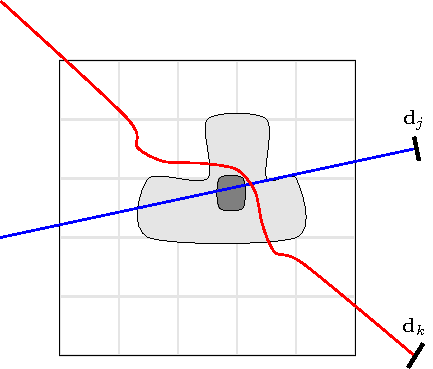
\includegraphics[width=0.45\linewidth]{MotionCorrection/diagrammotion1.pdf} 
\label{fig:fig21a} 
}
\subfigure[]{ 
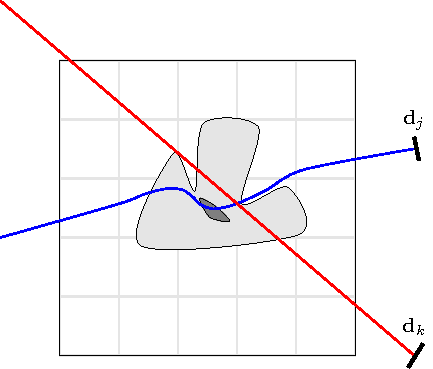
\includegraphics[width=0.45\linewidth]{MotionCorrection/diagrammotion2.pdf} 
\label{fig:fig21b} 
}
\caption{\label{fig:motion} The integral over a path in image (a) yields the same result as the integral over the same coloured path in the deformed image (b).} 
\end{center} 
\end{figure}



\subsection{Warped projection operator in a GPU}

The warped X-ray paths cannot be easily translated into classic projection operators.  Evaluating the length of a curvilinear path accurately inside every voxel it traverses would require a set of complex numerical methods which would inevitably increase the computation time significantly.  Instead, the uniformly sampled projection method explained in chapter 4 is used, for which the ray-warping operation becomes a straightforward modification of the code.  Rather than sampling at each image coordinate along a straight line, the vector field at that coordinate is first added and then the image is sampled.
 
The pseudocode in a GPU is outlined in algorithm \ref{alg:interp}.  One thread per X-ray is launched to compute $N_{ray}$ threads organized in divV$\times$divU blocks.  This means that instead of computing each of the path integrals in lexicographical order, small subsets of blocks (in the detector) are computed together.  This decreases the memory latency and increases the overall speed of the kernels by up to 300\% in our tests.  For more information about GPU memory access and optimal X-ray indexing we refer the reader to the work by Chou \emph{et al}\cite{Chou2011}.  As information about the texture cache is proprietory, empirical tests were made to find the best size for divV and divU.  These showed 32$\times$32 to be fastest on an NVIDIA Tesla 40k.  Note that there are reportedly faster structures for GPU kernels\cite{forwardproj}, but our tests showed no such improvement so we have stuck to the simplest approach of one thread per ray.

\begin{algorithm}

\caption{Motion interpolated X-ray projection
\label{alg:interp}}
\begin{algorithmic}[1]
\State{Precompute geometric constants}
\Launch{$N_{ray}$ threads organized in divU$\times$divV blocks}
    
\For{X-ray path}
      \State{Compute $[x,y,z]$ sample position}
      \State{Sample $[\textup{DVF}_x,\textup{DVF}_y,\textup{DVF}_z]= \textbf{DVF}(x,y,z)$}
      \State{Sum+= $\Delta l \cdot \textup{Image}(x+\textup{DVF}x,y+\textup{DVF}y,z+\textup{DVF}z)$}      
\EndFor
\EndKernel{} 
\end{algorithmic}

\end{algorithm}

Once an X-ray is selected, it is sampled over its path at every user-provided $\Delta l$ step length.  As previously mentioned, any real-valued coordinates, $p=[x,y,z]$, will yield a sample value using the interpolated read of texture memory.  The point is first sampled over the relevant DVF, yielding the change in coordinates of that specific point, then the image is sampled at the new displaced coordinates, $q=p+\textup{DVF}$.  The DVFs needed are those that describe the deformation from all the shifted states back to the reference one of the reconstruction.   Note that this description must be provided in the coordinate system of the reference state, so that $q-p$ is the extent of the inter-phase motion arriving at $p$ rather than originating from it.  This makes it more complicated than the forward mappings from the reference state to each of the others.



\subsection{Warped back projection operator in a GPU}

Warped back projection is simpler to compute as shown in the pseudocode outlined in algorithm \ref{alg:back}.  First, the standard back projection is computed using memory latency aware voxel ordering.  Then, a second GPU kernel is launched with the same thread and block sizes and, for each voxel, a sample of the relevant shifted image is taken at $(x+\textup{DVF}x,y+\textup{DVF}y,z+\textup{DVF}z)$.  This last step is basically a 3D interpolation.  It is important to note that the DVFs used here are not the same as those for projection.  And, although they are the inverse of each other, that inversion is not nearly as mathematically straightforward as a change of sign.

\begin{algorithm}

\caption{Motion X-ray back projection
\label{alg:back}}
\begin{algorithmic}[1]
\State{Precompute geometric constants}
\Launch{$N_{voxel}$ threads organized in divX$\times$divY$\times$divZ blocks}
    
      \State{Compute $[u,v]$ detector position in line with a source-voxel direction}
      \State{Sample Detector$(u,v)$}
      \State{Compute corresponding weight $w$}
      \State{WarpedImage$ = w *\textup{Detector}(u,v)$}  
      \Ensure{} 
      
      \Require{$N_{voxel}$ threads, organized in divX$\times$divY$\times$divZ blocks}
      \State{Sample $[\textup{DVF}_x,\textup{DVF}_y,\textup{DVF}_z]= \textbf{DVF}(x,y,z)$}
      \State{Image=  $\textup{WarpedImage}(x+\textup{DVF}x,y+\textup{DVF}y,z+\textup{DVF}z)$}      
\EndKernel{} 
\end{algorithmic}

\end{algorithm}

Several reportedly faster back projection operator structures exist in the literature.  We found that the one by Zinsser \textit{et al}\cite{zinsser2013systematic} can lead to execution speeds up to four times faster, but only when multiple back projections are used at the same time in the kernel.  Since the vector fields of the motion-compensated algorithm would generally be different for each back projection, this kernel structure will not acclerate the computation.  However, as the drawbacks of using the more complex structure are negligible, it has nevertheless been implemented in our code.  Thus, if a case is treated in which there is no motion to compensate, it will run more quickly.



\subsection{Motion-compensated algorithm}

Using any iterative CT reconstruction algorithm with warped projection and back projection is simple once the DVFs are known.  But first, a reference image is needed and the DVFs from this reference state to the shifted states must be computed, together with the inverse DVFs back to the reference. Once the DVFs are known, the only modifications to a given algorithm are minor.  Whenever the projection operator is used, the warped projection operator with the inverse DVFs should be used instead.  Likewise, for back projection, the warped version with the forward DVFs should replace the standard code.  This allows motion to be included in both operators inside any algorithm independently of the mathematics that invokes those operators.





\section{Results}

In order to validate the motion-compensation algorithm, two different tests were performed.  The results are presented in this section.  First, a proof of principle is established by subjecting a digital thorax phantom to a well-defined, if somewhat contrived deformation with time.  In this case, the expected image at any instant is perfectly known, but despite this the inverse motion map must still be computed numerically and is necessarily only approximate.  The motion moves all voxels within the image (but not the image boundaries) and the amplitude of the deformation is made substantially larger than any real movement in a breathing patient.  A second test is performed using clinical 4D-CT images, where the motion is only approximately known.  Nevertheless, even an approximate motion model can be exploited to significant beneficial effect.



\subsection{Arbitrary deformation of a digital phantom}

The phantom used is a digital representation\cite{xcatweb} of a human thorax comprising $256^3$ cubic voxels.  Motion is simulated according to equation \ref{eq:motion} using 100 equidistant discrete steps of an arbitrary time scale $t$, which runs from 0 to 1, and using $L=128$.  This creates a steadily increasing sinusoidal deformation in all three spatial dimensions, displacing all voxels throughout the volume of the phantom.  Only the boundaries at the faces of the cube and the three perpendicular mid-planes that intersect at its centre remain unshifted.  Figure \ref{fig:motion_Res2} shows a cross-section of the undeformed reference image at $t=0$ and of the deformed image at $t=1$.  Not only are there no static regions, but the deformation is huge compared with real breathing\cite{Liu2007531}, locally approaching three times that for a typical size of thorax.
\begin{eqnarray}
V(x,y,z) = \bigl(\nonumber\\
8*t*\sin(x \cdot \pi/L)\sin(y \cdot \pi/L)\sin(z \cdot \pi/L),\nonumber \\
8*t*\sin(x \cdot \pi/L)\sin(y \cdot \pi/L)\sin(z \cdot \pi/L),\nonumber\\
8*t*\sin(x \cdot \pi/L)\sin(y \cdot \pi/L)\sin(z \cdot \pi/L)\bigr)
\label{eq:motion}
\end{eqnarray}



\begin{figure}
\begin{center} 
\subfigure[]{ 
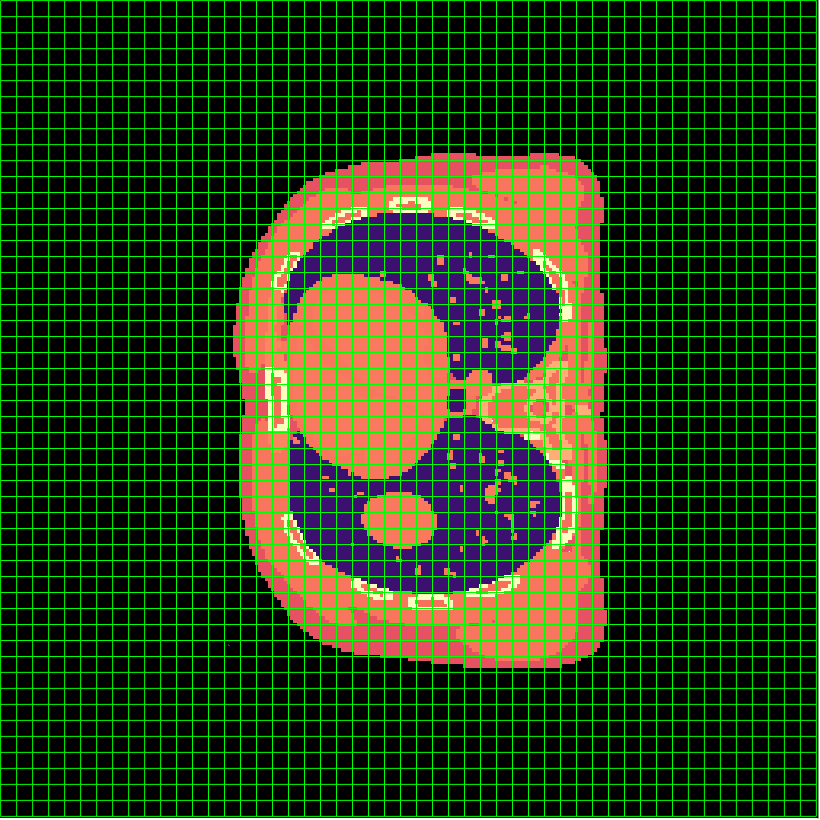
\includegraphics[width=0.415\linewidth]{MotionCorrection/thorax8XCAT.png} 
\label{fig:motion_Res2a} 
}
\subfigure[]{ 
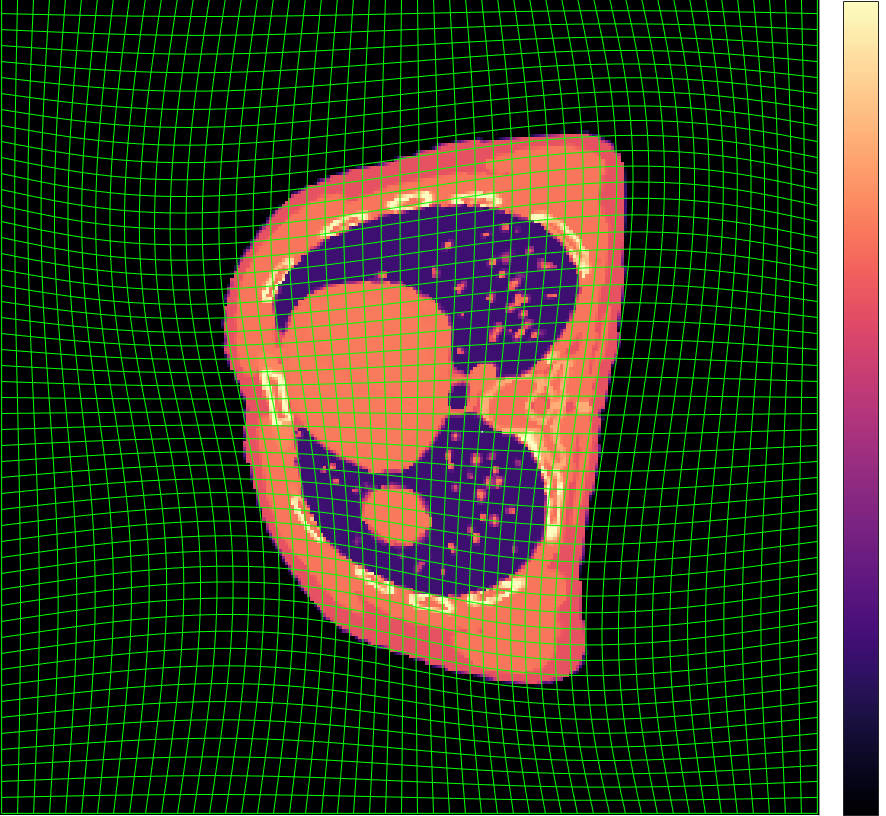
\includegraphics[width=0.45\linewidth]{MotionCorrection/thorax1XCAT.png} 
\label{fig:motion_Res2b} 
}
\caption{\label{fig:motion_Res2} Transverse plane of the thorax phantom (a) without deformation and (b) at maximum deformation.  A regular mesh overlay illustrates the motion map, although the actual voxels of the phantom are much smaller than this mesh size. The colour scale is linear attenuation coefficient in the range [0-0.045].} 
\end{center} 
\end{figure}

CBCT data are generated comprising 100 projections, one for each time step and covering a full circle.  In order to benchmark the results, 100 CBCT projections are also generated from the undeformed $t=0$ data alone, providing a comparable dataset for reconstruction but from which motion is entirely absent.  The images are reconstructed using 100 iterations of the SART algorithm.

Figure \ref{fig:result21} shows cuts of three different CBCT reconstructions of the reference state.  Motion is not included in the first and motion compensation is applied only in the last.  The latter reconstruction is qualitatively almost identical to the static one despite the necessarily approximate inverse deformation map.  However, the error in the inverse DVF, which is computed using a kernel splatting technique, is very small with more than 95\% of the errors less than 0.05 voxels in absolute distance.  This is typical of the numerical error that one can expect starting from a forward DVF that is well-known.

The error between the original phantom and each of the reconstructions is shown in figure \ref{fig:error2}.  The image in the uncompensated dynamic case is highly saturated in various places, whereas the motion-compensated image has only slightly higher error overall than the static reconstruction.  One would expect more iterations to reduce the error further.  Cuts in the other planes are found to be qualitatively very similar.

\begin{figure}[ht]
\begin{center}
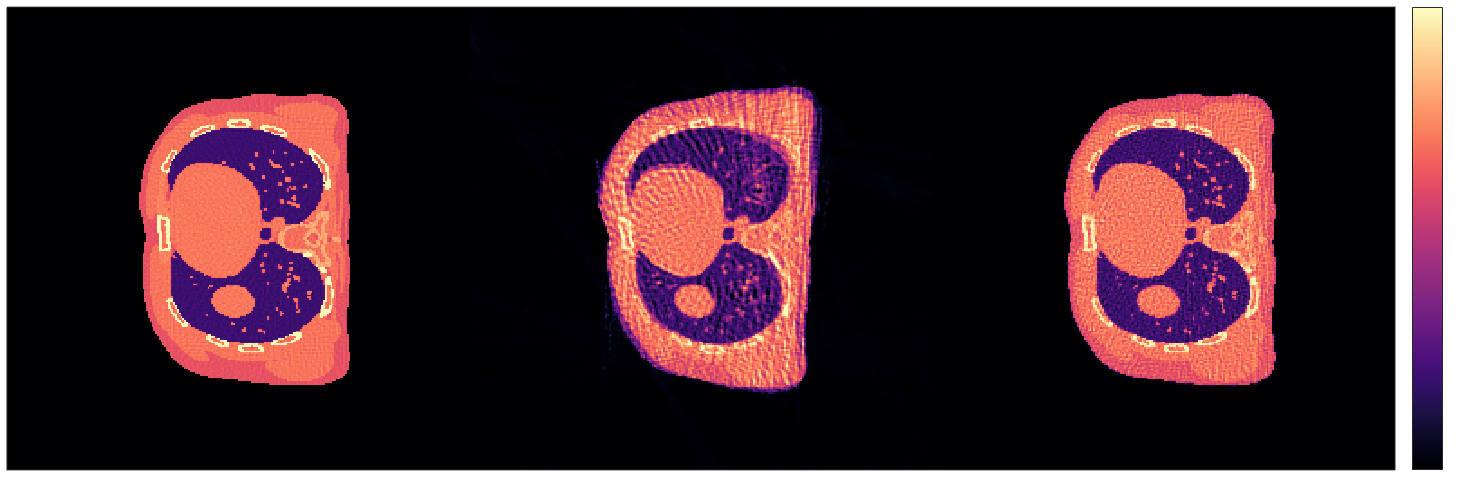
\includegraphics[width=1\linewidth]{MotionCorrection/motion2XCAT2.png}
\hspace{0.1cm}{\footnotesize (a)}\hspace{4.3cm}{\footnotesize (b)}\hspace{4.3cm}{\footnotesize (c)}
\caption{\label{fig:result21} Transverse cross-section of the CBCT reconstruction made (a) using SART in the absence of motion; (b) with motion using uncompensated SART; (c) with motion using compensated SART. The colour scale is linear attenuation coefficient in the range [0-0.045].} 
\end{center}
\end{figure}

\begin{figure}[ht]
\begin{center}
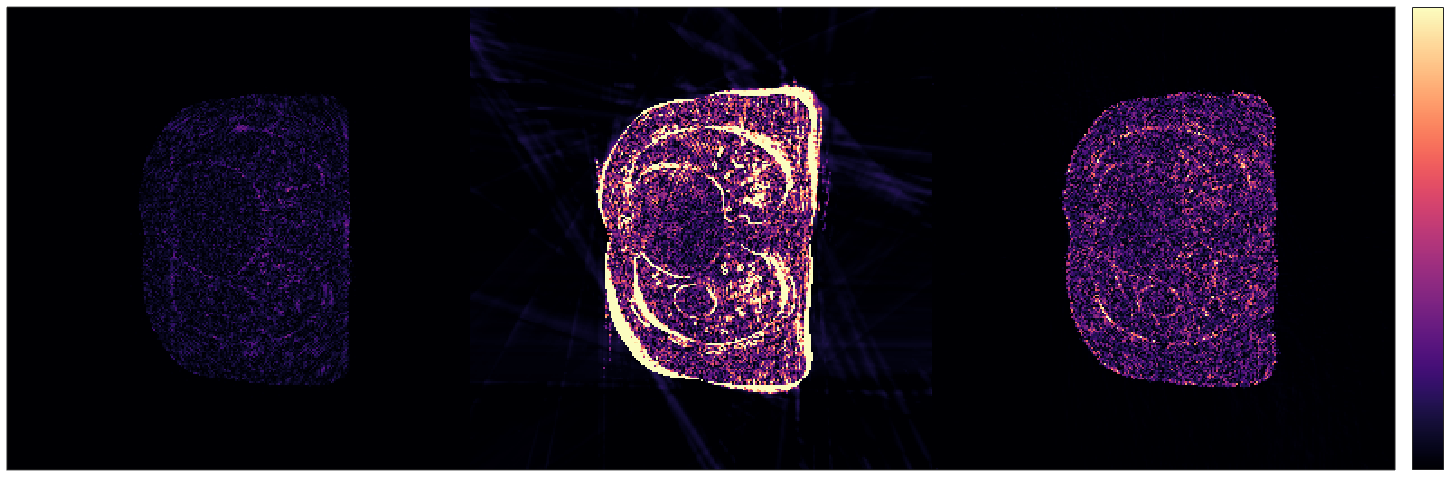
\includegraphics[width=1\linewidth]{MotionCorrection/motion21errorXCAT2.png}
\hspace{0.1cm}{\footnotesize (a)}\hspace{4.3cm}{\footnotesize (b)}\hspace{4.3cm}{\footnotesize (c)}

\caption{\label{fig:error2} Transverse cross-section of the difference between the known phantom (figure \ref{fig:motion_Res2a}) and the CBCT reconstruction made (a) using SART in the absence of motion; (b) with motion using uncompensated SART; (c) with motion using compensated SART.  The display range is significantly enhanced with respect to that of figure \ref{fig:result21}. The colour scale is linear attenuation coefficient in the range [0-0.01].} 
\end{center}
\end{figure}

Tellingly, the difference between the static reconstruction and the motion compensated one, as shown in figure \ref{fig:error23}, is quasi-uniform with no large differences at the boundaries between tissue types.  This means that, while the error may be larger in the motion-compensated case, it will not prevent the correct delineation of an organ or a tumour.

\begin{figure}[ht]
\begin{center}
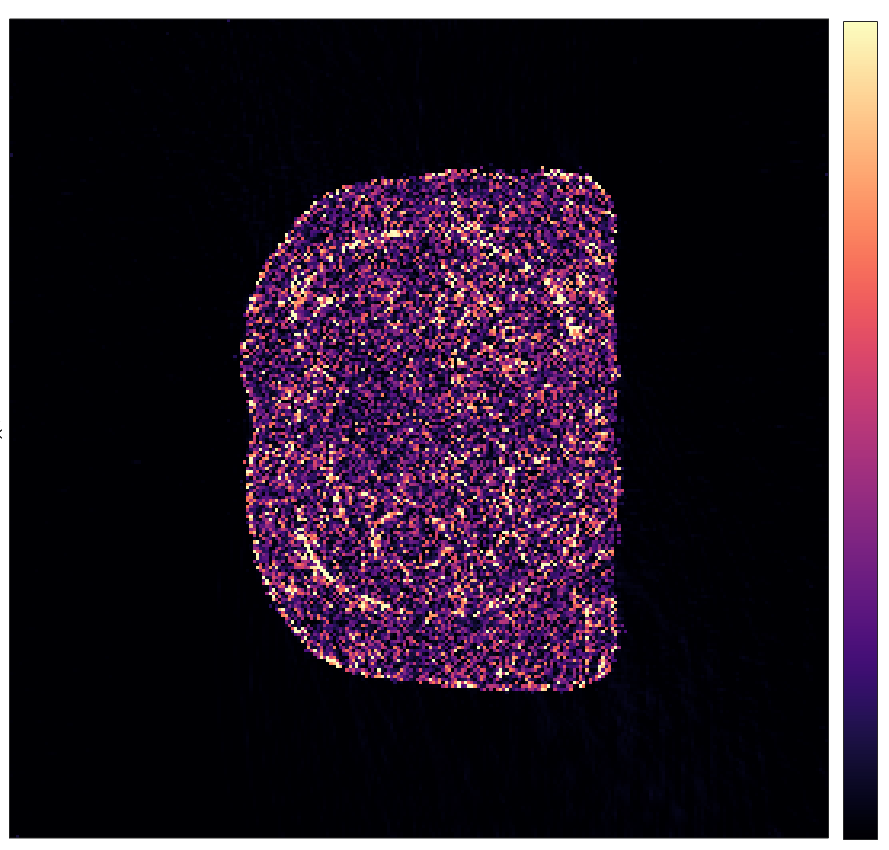
\includegraphics[width=0.6\linewidth]{MotionCorrection/motion2errorXCAT2.png} 
\end{center}
\caption{\label{fig:error23} Transverse cross-section of the difference between the static reconstruction of figure \ref{fig:error2}(a) and the motion-compensated one of figure \ref{fig:error2}(c). The colour scale is linear attenuation coefficient in the range [0-0.005].} 
\end{figure}

This test demonstrates that the new method can handle arbitrary, non-cyclic motion and that it works well even when the inverse deformation map is not perfectly known.


\FloatBarrier
\subsection{Real patient data}

The second test is performed using clinical data with precomputed DVFs, which are not entirely accurate.  It is important to note that no real CBCT data are used, only 4D-CT image data.  These are taken from the so-called POPI-model\cite{vandemeulebroucke2007popi} and are publicly available\cite{popi-modelweb}.  The data comprise ten 3D-CT images (labelled from ``0'' to ``9'') of the thorax equally spaced during the breathing cycle of a single patient.  Additionally, motion maps generated by two different methods are provided by the authors describing the inter-phase motion of the voxels.  We choose to use the maps that are generated by the parametric method for no specific reason as, statistically, both methods are reported to have similar errors.  And we choose to use the 3D-CT image labelled ``1'' as the reference state to be reconstructed because the authors provide the motion vectors from this state to all the others.  The reference state of the thorax can be seen in figure \ref{fig:realthorax}.  The particular feature of a tumour is highlighted.

%\begin{figure}[H]
%\begin{center} 
%\includegraphics[width=1\linewidth]{thoraxalmagma.png} 
%\caption{\label{fig:realthorax} 3D-CT scan of a lung radiation therapy patient at breathing phase ``1'' cut to show the tumour (located inside the green rectangle) in the (a) transverse, (b) coronal and (c) sagittal planes.  The colour scale is in arbitrary units.} 
%\end{center} 
%\end{figure}



% NOTE TO EDITOR: I tried to make the spacing between figures the smallest, but the
\begin{figure}[H]
\begin{center}
\hspace*{\fill} 
\subfigure[]{ 
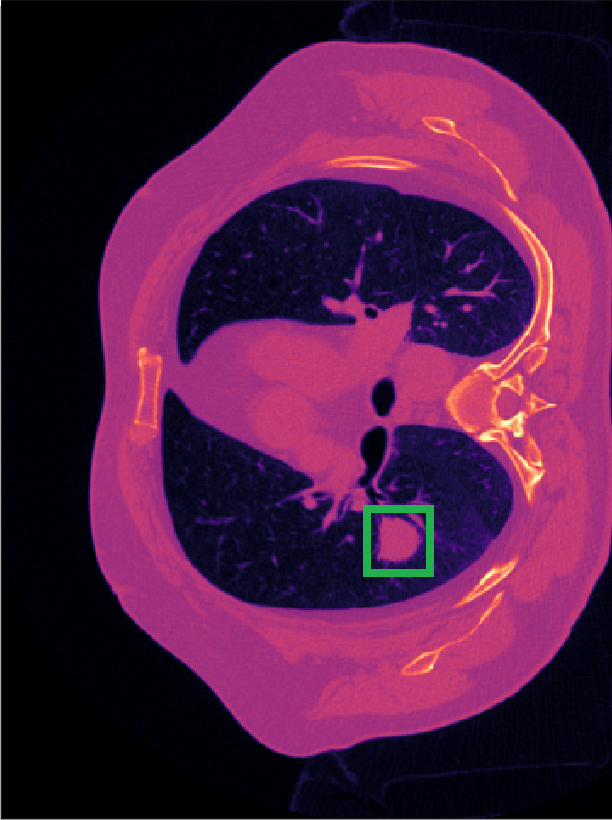
\includegraphics[scale=.2]{MotionCorrection/thoraxmagma_1.png} 
}\hfill
\subfigure[]{ 
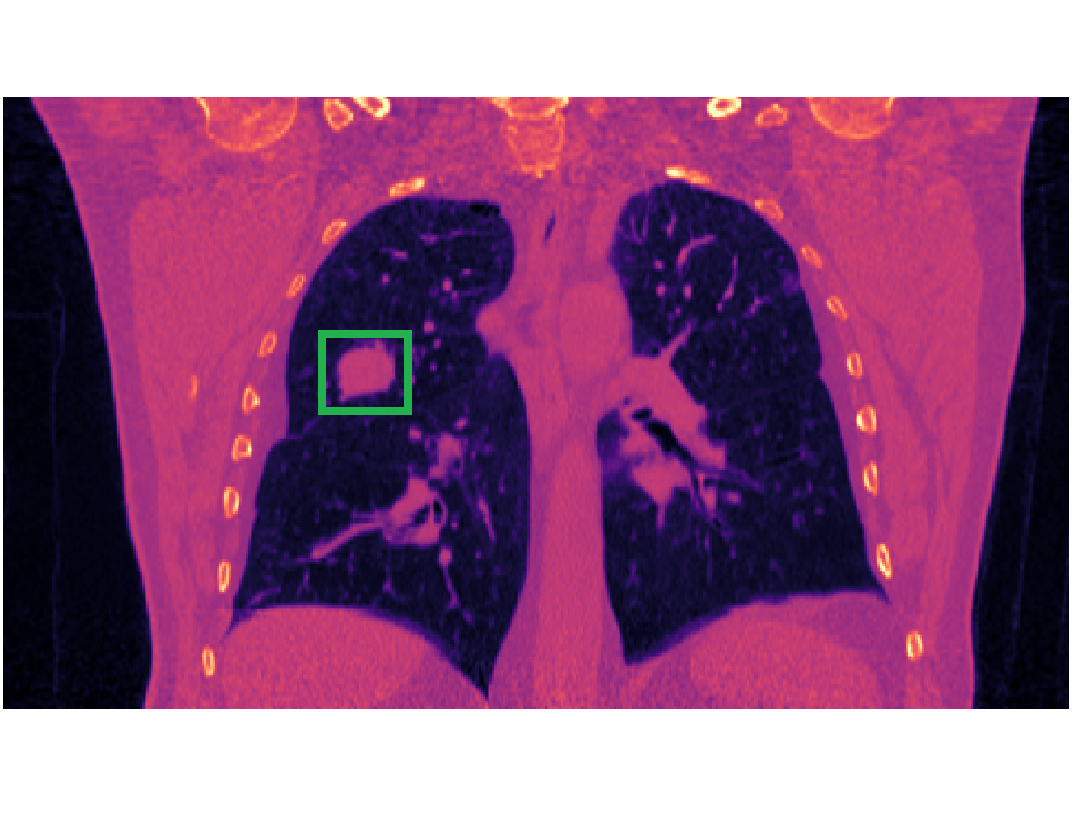
\includegraphics[scale=.2]{MotionCorrection/thoraxmagma_2.png} 
}\hfill
\subfigure[]{ 
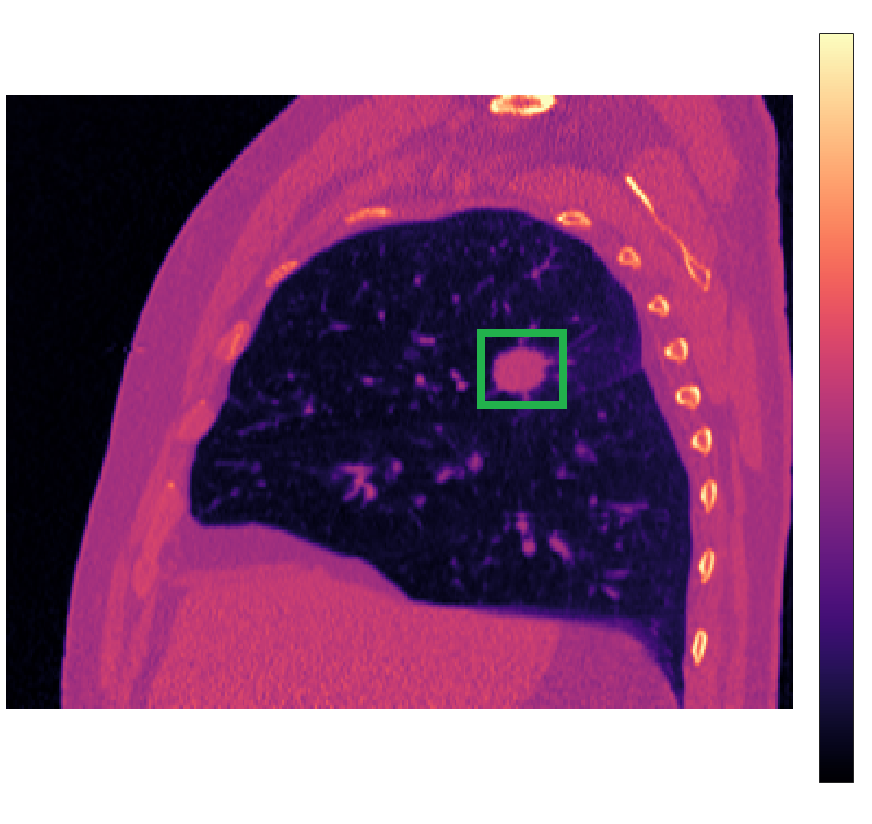
\includegraphics[scale=.2]{MotionCorrection/thoraxmagma_3.png} 
}\hfill
\hspace*{\fill} 

\caption{\label{fig:realthorax} 3D-CT scan of a lung radiation therapy patient at breathing phase ``1'' cut to show the tumour (located inside the green rectangle) in the (a) transverse, (b) coronal and (c) sagittal planes.  The colour scale is linear attenuation coefficient in the range [0-2000].} 
\end{center} 
\end{figure}



In order to simulate CBCT data, projections are generated from the phase-binned 3D-CT images.  No extra noise is added as the images themselves are already noisy.  \textcolor{black}{One hundred equally spaced projections covering a full circle are generated for each of the ten states and from these a subset is chosen, 10 from each breathing phase, to give 100 projections each 3.6 degrees apart and spanning a complete breathing cycle.}  Note that the DVFs are not used to approximate continuous movement as this would compromise the independence of the test that the quality of any subsequent motion-compensated reconstruction employing those DVFs affords.  In order to benchmark the results, 100 CBCT projections are simulated from the state ``1'' data alone, providing a comparable dataset for reconstruction but from which motion is essentially absent.

There are four significant error sources inherent in the original 4D-CT data before a CBCT reconstruction is even attempted.  There is that due to phase binning, which is particularly significant in the regions that move the most.  This is visible in figure \ref{fig:realthorax}, for example in the lower boundary of the lungs.  Another error source lies at the top and bottom (in the cranial-caudal direction) of the 3D-CT images.  Due to the original data acquisition and reconstruction techniques, the images have increased noise-like errors in their extrema and, because of the randomness of these errors, the images are not entirely consistent with each other in these regions.  The third main error in the source data is the inaccuracy of the DVFs in some areas.  Finally, the inverse of the DVFs will have additional errors due to the numerical method used to invert them.

Given these numerous sources of error, one can expect streak artifacts in addition to the usual random noise exhibited in any reconstruction.  As previously mentioned, it is a strength of the new motion-compensation method that it can be applied to any iterative algorithm, so one can be employed that reduces such artifacts by, for example, minimizing the total variation (TV).  We elect to use both the well-known SART and the TV algorithm ASD-POCS\cite{ASD_POCS} in this test.

Figure \ref{fig:res3} shows cuts of four different CBCT reconstructions of the reference state.  Motion is included in all except the first, but motion compensation is applied in only the last two.  The SART algorithm is used in all cases except the last, which is processed with ASD-POCS.  The second, uncompensated image has lost much of the detail inside the lungs, while the compensated algorithms, even with all the errors in the DVFs and data, reconstruct the tissue boundaries inside the thorax with higher accuracy.  The last, TV case is particularly good.  This is even more evident in figure \ref{fig:res3err}, where the difference between the original 3D-CT image and each reconstruction is shown.  One can see that the error is smaller overall in the motion-compensated cases, for which the discrepancy where the tumour is located is barely visible.  Cuts in the coronal plane, which is the one containing the largest movement of the lungs, underscore the remarkable improvement in the motion-compensated images (see figures \ref{fig:tumourCC} and \ref{fig:tumourCC_err}).

\begin{figure}[H]
\begin{center} 

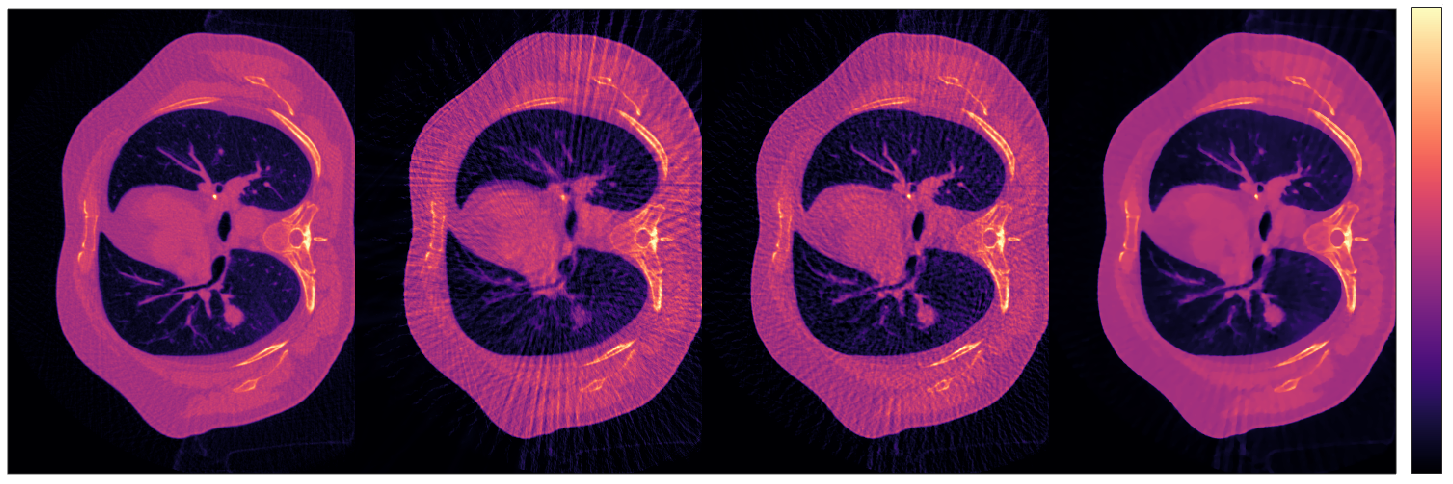
\includegraphics[width=1\linewidth]{MotionCorrection/res32.png} 
\hspace{0.1cm}{\footnotesize (a)}\hspace{3.2cm}{\footnotesize (b)}\hspace{3.2cm}{\footnotesize (c)}\hspace{3.2cm}{\footnotesize (d)}

\caption{\label{fig:res3}  Transverse cross-section of the CBCT reconstruction made (a) using SART in the absence of motion; (b) with motion using uncompensated SART; (c) with motion using compensated SART; (d) with motion using compensated ASD-POCS. The colour scale is linear attenuation coefficient in the range [0-2000].} 
\end{center} 
\end{figure}

\begin{figure}[H]
\begin{center} 
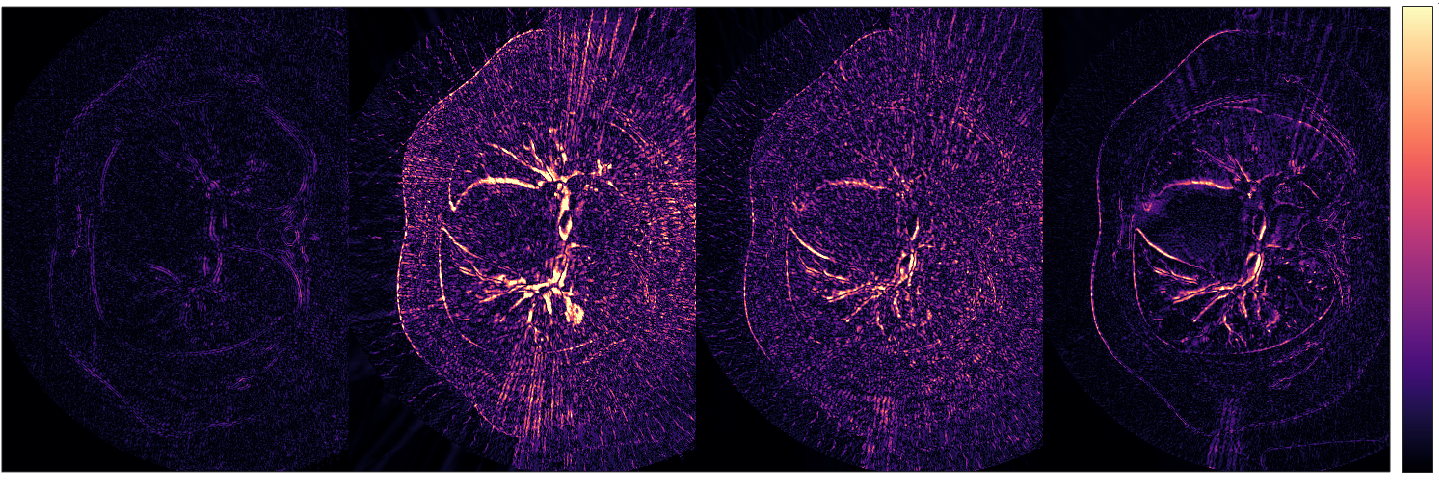
\includegraphics[width=1\linewidth]{MotionCorrection/res3err2.png} 
\hspace{0.1cm}{\footnotesize (a)}\hspace{3.2cm}{\footnotesize (b)}\hspace{3.2cm}{\footnotesize (c)}\hspace{3.2cm}{\footnotesize (d)}
\caption{\label{fig:res3err}  Transverse cross-section of the difference  between the original 3D-CT image (figure \ref{fig:realthorax}(a)) and the CBCT reconstruction made (a) using SART in the absence of motion; (b) with motion using uncompensated SART; (c) with motion using compensated SART; (d) with motion using compensated ASD-POCS. The colour scale is linear attenuation coefficient in the range [0-400].} 
\end{center} 
\end{figure}

\begin{figure}[H]
\begin{center} 
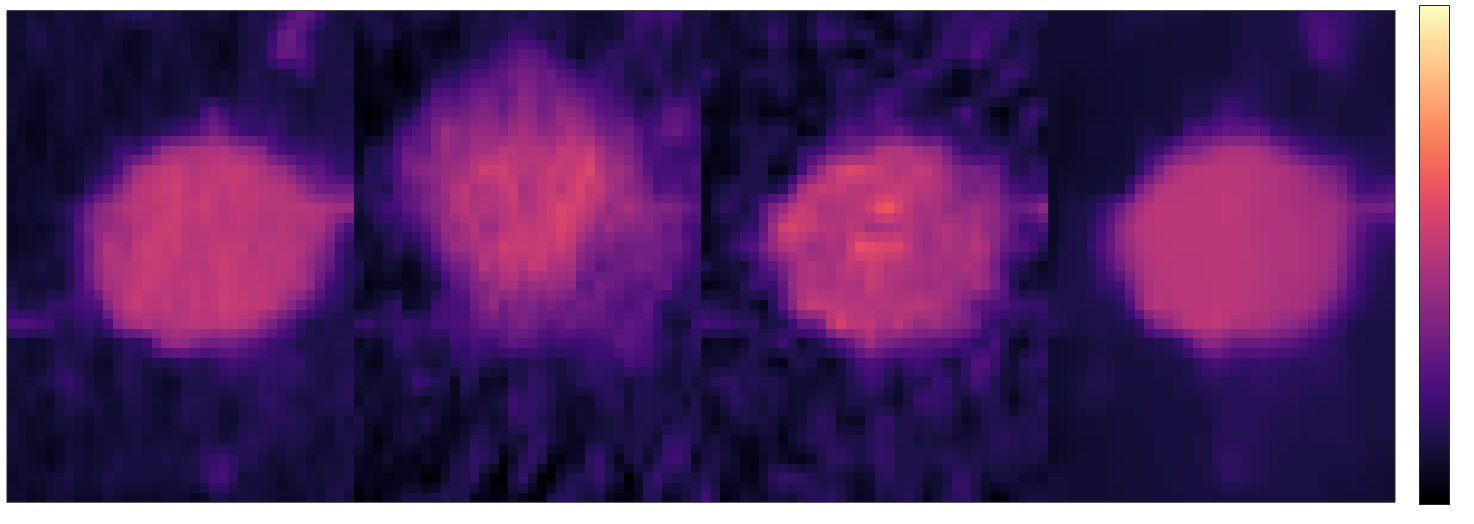
\includegraphics[width=1\linewidth]{MotionCorrection/tumourCC2.png}
\hspace{0.1cm}{\footnotesize (a)}\hspace{3.2cm}{\footnotesize (b)}\hspace{3.2cm}{\footnotesize (c)}\hspace{3.2cm}{\footnotesize (d)} 
\caption{\label{fig:tumourCC}  Zoom on the region where the tumour is located in a coronal cross-section of the CBCT reconstruction made (a) using SART in the absence of motion; (b) with motion using uncompensated SART; (c) with motion using compensated SART; (d) with motion using compensated ASD-POCS. The colour scale is linear attenuation coefficient in the range [0-2000].} 
\end{center} 
\end{figure}

\begin{figure}[H]
\begin{center} 
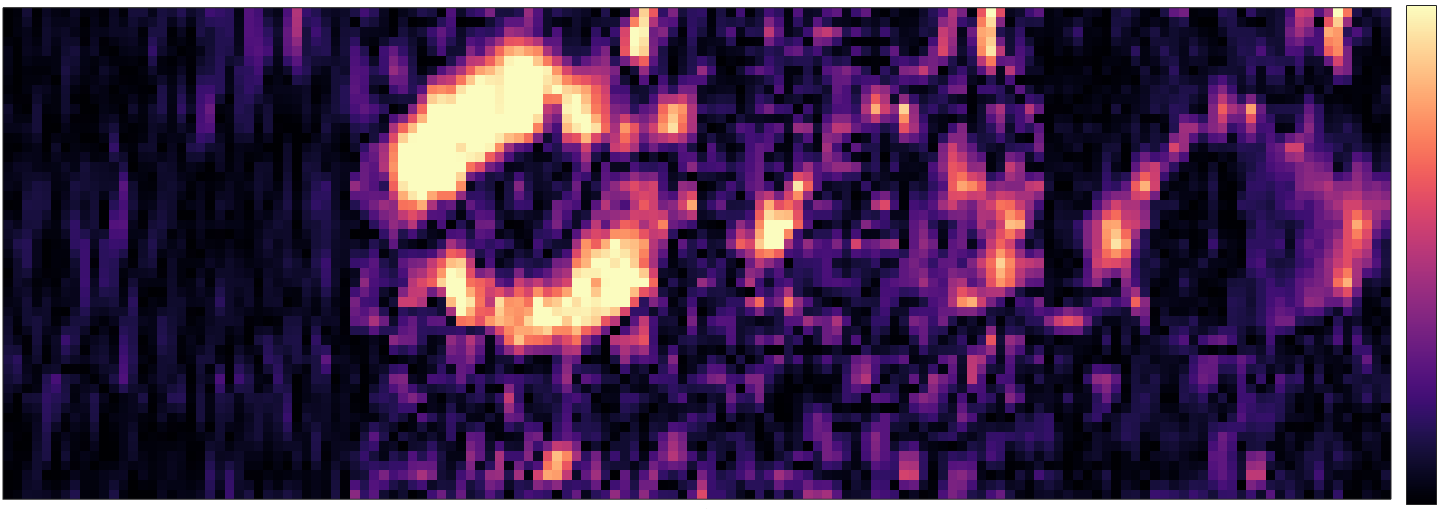
\includegraphics[width=1\linewidth]{MotionCorrection/tumourCC_err2.png}
\hspace{0.1cm}{\footnotesize (a)}\hspace{3.2cm}{\footnotesize (b)}\hspace{3.2cm}{\footnotesize (c)}\hspace{3.2cm}{\footnotesize (d)} 
\caption{\label{fig:tumourCC_err}  Zoom on the region where the tumour is located in a coronal cross-section of the difference  between the original 3D-CT image (figure \ref{fig:realthorax}) and the CBCT reconstruction made (a) using SART in the absence of motion; (b) with motion using uncompensated SART; (c) with motion using compensated SART; (d) with motion using compensated ASD-POCS. The colour scale is linear attenuation coefficient in the range [0-400].} 
\end{center} 
\end{figure}


For a more quantitative assessment, the resultant images are cropped around the tumour taking a 36$\times$36$\times$26 subset of voxels in the anterior-posterior, lateral and cranial-caudal directions (as indicated by the green rectangles in figure \ref{fig:realthorax}).  Then, in order to evaluate the quality of the reconstruction inside this box, three different indices are used to compare the original 3D-CT image with the four CBCT reconstructions of this test.

\begin{itemize}

\item Root Mean Square Error (RMSE) is defined
\begin{equation}
\boldsymbol{\textrm{RMSE}}=\sqrt{\frac{\sum_{n=1}^N(\hat{p}_n-p_n)^2}{N}},
\end{equation}
where $\hat{p}_n$ is a voxel in the original image, $p_n$ a voxel in the reconstructed one and $N$ is the number of voxels.  A larger value means more difference.

\item Universal Quality Image (UQI)\cite{wang2002universal} is a widely used index and is defined
\begin{equation}
\boldsymbol{\textrm{UQI}}=\frac{2\textrm{cov}(\hat{\mu},\mu)}{\hat{\sigma}^2+\sigma^2}\cdot \frac{2\hat{\mu}\mu}{\hat{\mu}^2+\mu^2},
\end{equation}
where $\textrm{cov}$ is the covariance function and $\hat{\mu},\mu$ are the means and $\hat{\sigma}^2,\sigma^2$ the variances of the original and reconstructed images, respectively.  UQI yields a value between 0 and 1, increasing with increasing similarity.

\item Segmentation mismatch.  A segmentation value using Otsu's method\cite{otsu1975threshold} is computed for the original image and all voxels in the reconstructed image are identified as lying inside or outside the tumour according to that value.  Then the number of voxels that are mislabelled by that segmentation is counted.  A larger value means more difference.

\end{itemize}

The results for each index applied to the subset of voxels in the region of the tumour is shown in table \ref{tab:quality}.  As expected, the SART reconstruction even in the absence of motion in the data does not reproduce the original image with any great accuracy as the data are still not perfect and CBCT reconstruction has its limitations.  Nevertheless, it is a sufficiently good reconstruction to take as a benchmark for the others.  Indeed, it should be stressed that, although the CBCT data here are artificial, in a practical scenario the equivalent static dataset would require a full order of magnitude more radiation dose to acquire than the dynamic one because of phase binning.  In comparison with this static CBCT case, uncompensated SART applied to the dynamic data has considerably worse reconstruction quality, missing almost 10\% of the tumour by segmentation.  Motion-compensated SART performs significantly better, getting closer to the static SART values.  Finally, the motion-compensated ASD-POCS results are very similar to those of the reconstruction without any motion.  One would expect more advanced TV algorithms to perform even better.
  
\begin{table}[H]
\begin{center}
\caption{Tumour reconstruction quality by different algorithms}
\label{tab:quality}
\begin{tabular}{|l|| c | c | c |}
\hline
 & RMSE & UQI & Seg. mismatch \\
\hline \hline  
 SART without motion & 67.18 & 0.9656 & 1108 (3.288\%)\\
 SART with motion & 172.12 & 0.7617 & 3315 (9.838\%)\\
 SART motion-compensated & 109.84 & 0.9077 & 1505 (4.466\%)\\
 ASD-POCS motion-compensated & 82.72 & 0.9451 & 1284 (3.811\%)\\
\hline  
\end{tabular}
\end{center}
\end{table}

This test demonstrates that the new method can be used in a clinical context even if the motion due to breathing is only approximately known.



\subsection{Computation times}
\textcolor{black}{An important factor for clinical feasibility is the computation time that motion compensation adds to a standard reconstruction. The kernel times have been measured on a TESLA k40 GPU and are reported for the projection and back projection operations both with and without motion compensation. Two variants of the back projection operation have been tested, the single- and the dual-kernel versions as described in algorithm \ref{alg:back}. Table \ref{tab:times} lists computation times for $512\times 512 \times 141$ image and DVF sizes and a $512^2$ detector size. The reported times are the average of 100 calls and only account for kernel time. As the back projection kernels are optimized for multiple calls, the average computation times for a single update or a multiple update are different. Both these times are shown in the back projection columns of Table \ref{tab:times}. Reducing the size of the DVFs hardly changes the computation time as the number of samples needed is determined by the image size alone.}

\textcolor{black}{Both the single- and dual-kernel back projection operations lead to similar reconstructed image quality, with a visually imperceptible improvement in the dual-kernel case (0.1 in RMSE). The dual-kernel approach is expected to be better as errors in the DVFs are amplified by the divergent cone angle in the single-kernal case.}

\begin{table}[H]
\begin{center}
\caption{GPU kernel times per projection.}
\label{tab:times}
\begin{tabular}{|l|| c | c | c |}
\hline
& Projection & \thead{Single-kernel \\Backprojection} & \thead{Dual-kernel\\ Backprojection}\\  
\hline
\hline
Standard& 6.5ms& 4ms/2.5ms&-\\   
Motion warped&120ms &24ms/18ms &13ms/3ms\\
\hline  
\end{tabular}
\end{center}
\end{table}

\section{Discussion}

We have demonstrated a significant improvement in CBCT image quality by removing motion artifacts using a modelling approach to motion compensation.  The resultant images still have some error compared with a static reconstruction, but critically, tissue boundaries are resolved with much greater accuracy than when motion is ignored. 

One of the greatest strengths of the new method is that it employs all the projection data to reconstruct an image, reducing the X-ray dose to the patient.  It is also completely algorithm independent; its novelty lies in a modelling approach, which in principle can be applied in conjunction with any static reconstruction algorithm.  In fact, most of the motion-compensation ideas present in the literature and reviewed at the beginning of this work could incorporate the method.  As some of these rely on refining DVFs, then, instead of using those DVFs to generate a deformed image from a prior high-quality one, they could be used to reconstruct images from the real acquired data.  Others rely on temporal reconstruction constraints, where the images at successive time steps are regularized to look similar to their neighbours.  Again, such techniques can be used in combination with the new motion compensation because the latter permits any state of the motion to be reconstructed.  Indeed, one could generate an X-ray video of the patient breathing if enough time steps are reconstructed and, as these frames are computationally independent, they could be processed in parallel.  And none of these extra images would require any extra dose for the patient.

The use of DVFs can lead to large memory requirements and an increased preprocessing time, but it has been established in phase space tomography that it is possible to trade off the accuracy of the maps against an increased number of iterations and that some parameters in the motion model itself can be refined by their influence on convergence\cite{pst1}\cite{pst2}.  More speculative is the idea of "bootstrapping" the DVFs without starting from any high-resolution images.  One can imagine repeatedly subdividing the CBCT data into more and more motion phases, and thus iterating both the images and the DVFs themselves at each subdivision, whilst still using all the data for each reconstruction by interpolating between DVFs until there are enough of these to describe the motion in sufficient detail.  This would be very heavy computationally and there is no guarantee of convergence.

As presented here, the method takes only 2 to 3 times longer than a standard iterative reconstruction algorithm due to the use of GPUs for the motion-compensated projection and back projection operators.  So the computational penalty is not large.  It is important to note that we used DVFs of the same size as the images (they are generally smaller) and the code was not highly optimized.  Careful tuning should lead to appreciably faster execution.

\textcolor{black}{One drawback of the method in an eventual clinical scenario is the need for a sufficiently accurate DVF for each of the projections. Obtaining realistic patient-specific DVFs is non-trivial.  However, statistical analysis\cite{Sonke2008590}\cite{0031-9155-51-17-003} has shown that, while inter-patient motion variability is high, intra-patient variability is low provided the patient performs free breathing.  And preliminary tests of DVF error tolerance of the motion compensation method suggest that the algorithm is very robust to undersampled and noisy DVFs due to its iterative nature, but futher study is required.  Additionally, a method that maximizes the quality of the DVFs needs to be identified. Obtaining the breathing amplitude using the Amsterdam Shroud\cite{0031-9155-58-5-1447} and correlating that with prior DVFs or with DVFs obtained using binned, low-resolution 4D-CBCT images from the same dataset are promising techniques.}

We consider that this motion compensation method could have a genuine impact in IGRT even though it is not yet at a clinical stage.  Better diagnostic imaging offers the prospect of less collateral damage to healthy tissue and increased survival rates.  Ultimately, it might be possible to steer a particle therapy beam in real time to follow a moving target. 



	
%\section{Conclusions}
%A novel approach to motion-compensated CT imaging has been demonstrated that uses the entire dynamic set of acquired data to reconstruct an image that is effectively rendered static, thereby considerably reducing motion artefacts.  This introduces the possibility of a significant reduction in radiation dose during imaging and treatment.  The method requires a knowledge of the deformation vector fields describing the motion between the reconstructed state and all others during the acquisition time span.  It removes much of the unwanted artefacts due to motion even when that knowledge is imperfect.  The method can be used in combination with most, if not all, existing static and 4D iterative reconstruction techniques.  Motion compensation based on these ideas is being rolled out to the algorithms available from the open-source TIGRE Toolbox\cite{TIGREweb}.  The potential clinical benefits are clear.



%\section{Acknowledgements}
%The authors would like to thank EPSRC for helping to fund this PhD work and NVIDIA for the hardware donation of a GPU.  Special thanks go to Robert Bryll and Imanol Luengo for interesting discussions and for speeding up the GPU code.
